\section{Cloud Infrastruktur}

Das Trainieren eines \textit{Deep Learning} Modells ist gerade bei großen CNN Architekturen äußerst rechenaufwendig. Tensor Operationen wie Matrixmultiplikationen und Konvolutionen erfordern im Rahmen des maschinellen Lernens hohe Parallelisierung und Taktfrequenzen, um in absehbarer Zeit gute Ergebnisse zu liefern. Die Rechenkapazität normaler Desktop-PCs reicht demnach meist nicht aus, um performantes \textit{Deep Learning} betreiben zu können. 

Abhilfe bieten Software-as-a-Service (SaaS) bzw. Platform-as-a-Service (PaaS) Angebote wie \textit{Amazon SageMaker}, \textit{Google Cloud Platform Cloud AI}, \textit{Azure ML Services} oder Start-ups wie \textit{FloydHub}. Diese bieten Infrastruktur in unterschiedlichen Zonen je nach Standpunkt der Rechenzentren zum Trainieren an sowie eine Plattform zum Verwalten der \textit{Deep Learning} Prozesse. 

\subsection{Trainingshardware}

Gerade GPUs bieten sich aufgrund ihres hohen Parallelisierungsvermögens gegenüber herkömmlichen CPUs an. Insbesondere \textit{NVIDIA} nimmt hierbei eine Vorreiterrolle in der Produktion von Server-GPUs ein. Die \textit{Compute Unified Device Architecture} (CUDA) von \textit{NVIDIA} ermöglicht hierbei als Programmiermodel und parallele Computing Plattform das Auslagern von Rechenprozessen auf GPUs. Das \textit{CUDA} Toolkit beinhaltet GPU beschleunigte Bibliotheken, einen Compiler, Entwicklungswerkzeuge sowie die eigentliche \textit{CUDA} Laufzeit und wird von vielen \textit{Deep Learning} Bibliotheken genutzt, wie z.B. \textit{PyTorch}. \cite{NVIDIA.20200209} \cite{PyTorch.20200209}

Vergleich man gängige GPUs, die oft in Rechenzentren der Hyperscaler angeboten werden, so ergibt sich folgende Tabelle \cite{TechPowerUp.20200209}:

\begin{tabular}[h]{l|c|c|c|c|c|c}
	& GTX 1080 & TITAN RTX & Tesla K80 & Tesla P100 & T4 & V100 \\
	\hline
	CUDA Cores & 2560 & 4608 & 2496 & 3584 & 2560 & 5120 \\
	Tensor Cores & / & 576 & / & / & 320 & 640 \\
	TFLOPS\footcite{Single Precision} & 8.873 & 16,31 & 4.113 & 9.526 & 8.141 & 14,13 \\
	Memory Bandwidth\footnote{in GB/sec} & 320,3 & 672 & 240,6 & 732,2 & 320 & 897 \\
	Max Power Consumption\footnote{During Normal Operation} & 180 & 280 & 300 & 250 & 70 & 300 \\
	\label{gpus}
\end{tabular}

Neben GPUs existieren seit 2015 die von Google entwickelten \textit{Tensor Processing Units} (TPUs). Diese Art von Spezialhardware erreicht pro TPU-Kern eine Rechenleistung von bis zu 92 TOPS \cite{HaraldBogeholz.20170406}. Schließt man 2048 solcher TPU-kerne zu einem TPU-Pod zusammen, so ergibt sich eine Rechenleistung von über 100 PetaFLOPS \cite{GoogleCloud.20200209}. 

\begin{figure}[ht]
	\begin{center}
		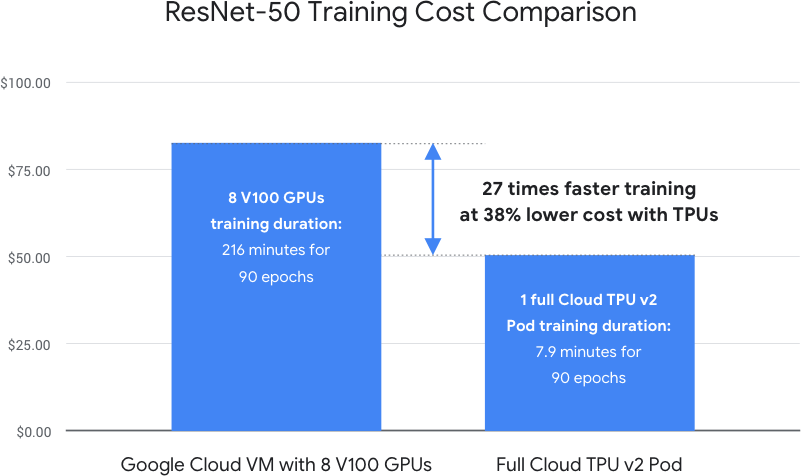
\includegraphics[width=14cm]{Bilder/tpu_comparison.png} 
		\caption[Vergleich V100 - TPU Pod]{Vergleich V100 - TPU Pod \cite{GoogleCloud.20200209b}}
		\label{tpu}
	\end{center}
\end{figure}

Eine weitere Steigerung versprechen Microsofts Field Programmable Gate Arrays (FPGAs), die allerdings nicht weiter im Rahmen dieser Arbeit betrachtet werden sollen \cite{KarlFreund.20170828}.

\subsection{FloydHub}

To be continued